%!TEX program = xelatex
\documentclass[UTF8,aspectratio=169,10pt,t]{ctexbeamer}

\mode<presentation> {
\usetheme{Madrid}
\setbeamertemplate{footline}[frame number] %设置页码
\setbeamercolor{page number in head/foot}{fg=blue} %设置页码颜色
\setbeamertemplate{navigation symbols}{} %去除控件
}
\usepackage{indentfirst}
\setlength{\parindent}{2em}
\usepackage{listings}
\usepackage{wrapfig}
\usepackage{graphicx}
%设置图片存放路径
\graphicspath{{figures/}}
\usepackage{multicol} %多列布局

%用户自定义区块环境
\usepackage{setspace}
\definecolor{hanblue}{rgb}{0.27, 0.42, 0.81}
\definecolor{indiagreen}{rgb}{0.07, 0.53, 0.03}
\definecolor{indianred}{rgb}{0.8, 0.36, 0.36}
\definecolor{indianyellow}{rgb}{0.89, 0.66, 0.34}
\definecolor{babypink}{rgb}{0.96, 0.76, 0.76}
\definecolor{ao(english)}{rgb}{0.0, 0.5, 0.0}
% \setbeamerfont{block title}{size=\small}
% \setbeamerfont{block body}{size=\small}
\setbeamerfont{block title}{}
\setbeamerfont{block body}{}
\newenvironment<>{blueblock}[1]{
    \setbeamercolor{block title}{fg=white,bg=hanblue}
    \begin{block}#2{#1}}{\end{block}}
\newenvironment<>{greenblock}[1]{
    \setstretch{1.3}\setbeamercolor{block title}{fg=white,bg=indiagreen}
    \begin{block}#2{#1}}{\end{block}}
\newenvironment<>{redblock}[1]{
    \setstretch{1.3}\setbeamercolor{block title}{fg=white,bg=indianred}
    \begin{block}#2{#1}}{\end{block}}
\newenvironment<>{yellowblock}[1]{
    \setstretch{1.3}\setbeamercolor{block title}{fg=white,bg=indianyellow}
    \begin{block}#2{#1}}{\end{block}}

\lstset{language=C++,
columns=flexible,
basicstyle=\footnotesize\ttfamily,                                      % 设定代码字体、大小
%numbers=left,xleftmargin=2em,framexleftmargin=2em,                   % 在左侧显示行号
%numberstyle=\color{darkgray},                                        % 设定行号格式
keywordstyle=\color{blue},                                            % 设定关键字格式
commentstyle=\color{ao(english)},                                     % 设置代码注释的格式
stringstyle=\color{brown},                                            % 设置字符串格式
%showstringspaces=false,                                              % 控制是否显示空格
%frame=lines,                                                         % 控制外框
breaklines,                                                           % 控制是否折行
postbreak=\space,                                                     % 控制折行后显示的标识字符
breakindent=5pt,                                                      % 控制折行后缩进数量
emph={size\_t,array,deque,list,map,queue,set,stack,vector,string,pair,tuple,unique\_ptr}, % 非内置类型
emphstyle={\color{teal}},
escapeinside={(*@}{@*)},
}

\title[\textit{Qt编程基础}]{Qt编程基础}

% \author
%     []
%     {}

\date{}

% \institute
%     {}


\begin{document}

\maketitle

\begin{frame}{目录}
\tableofcontents
\end{frame}

\begin{frame} {前言}
    \begin{yellowblock}{学习目标}
        \begin{enumerate}
            \item 掌握Qt开发环境的基本使用
            \item 了解基本的window界面框架
            \item 理解信号与槽机制
            \item 理解事件机制
            \item 理解模型/视图结构
            \item 学会简单动画绘图
        \end{enumerate}
    \end{yellowblock}
\end{frame}

\section{Qt简介}

\begin{frame}[fragile]{1~Qt简介}
\vspace{-3mm}
   \begin{block}{跨平台C++图形用户界面应用程序开发框架}
  \begin{itemize}
    \item 它既可以开发GUI程序,也可用于开发非GUI程序,比如控制台工具和服务器。
    \item Qt是面向对象的框架,使用元对象编译器生成扩展代码,易于扩展,允许组件编程。
  \end{itemize}
   \end{block}
\vspace{-2.3mm}
    \begin{columns}[T]
        \column{0.5\textwidth}
        \pause \centering 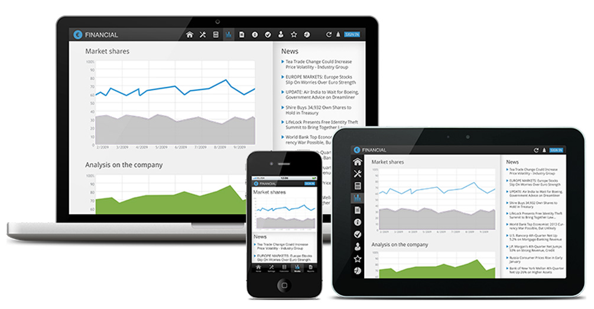
\includegraphics[width=0.66\textwidth]{fig/fig1} \vspace{-2.3mm}
   \begin{block}{跨平台}
 桌面OS:Windows, Linux, Mac; 移动OS:iOS, Android,WP; 嵌入式OS: QNX,VxWorks
  \end{block}
  \column{0.45\textwidth}
   \pause
 \centering 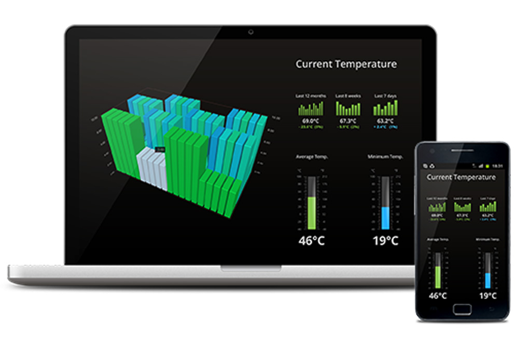
\includegraphics[width=0.58\textwidth]{fig/fig2}\vspace{-2.3mm}
   \begin{block}{集成开发平台}
 Design, Code, Debug \& Deploy Quickly\\
 ~~
  \end{block}
  \end{columns}
  \vspace{2mm}
\pause
\noindent \parbox{\textwidth}{应用:WPS、Skype、豆瓣电台、虾米音乐、暴雪的战网客户端、VirtualBox、Opera、咪咕音乐、\\Google地图、Adobe Photoshop Album}
\end{frame}

\begin{frame}[fragile]{1~Qt简介}
	\begin{block}{软件下载}
		\begin{description}
			\item[Qt版本] Qt 5
		\end{description}
	\end{block}
	\pause
	\begin{block}{在线教程}
		\begin{itemize}
			\item http://www.devbean.net/2012/08/qt-study-road-2-catelog/
			\item http://doc.qt.io/qt-5/gettingstarted.html
			\item http://doc.qt.io/qt-5/examples-widgets.html
		\end{itemize}
	\end{block}	
\end{frame}

\section{使用Qt}

\begin{frame}[fragile]{2~使用Qt}
(1) 创建 Hello World Qt!
		{\begin{figure}
			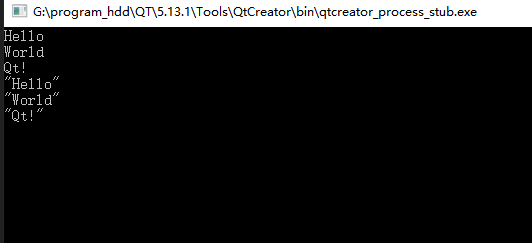
\includegraphics[width=0.6\textwidth]{fig/hello_word_qt.png}
		\end{figure}}
\end{frame}

\begin{frame}[fragile]{2~使用Qt}
	(2) 使用\alert{信号}与\alert{槽}机制实现简单的对象间通讯
	\begin{figure}
		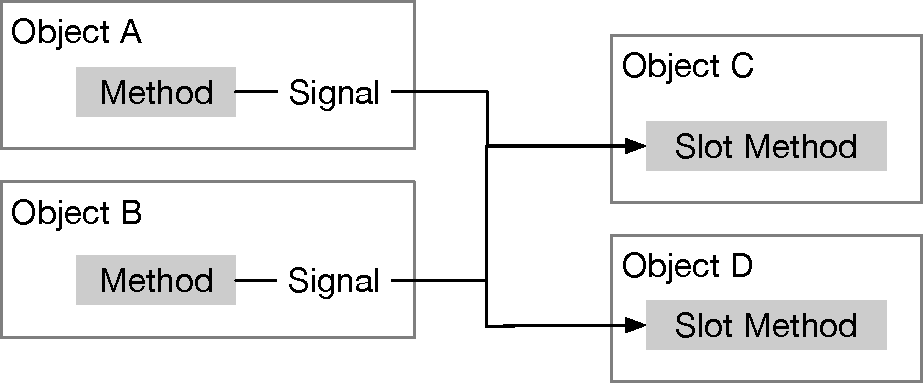
\includegraphics[width=0.45\textwidth]{fig/signals_slots.pdf}
	\end{figure}
			\pause
	\vspace{-7mm}
	\begin{columns}
		\column{0.48\textwidth}
		\begin{block}{信号 \texttt{signals}}
			\begin{itemize}
				\item 信号由对象发射
				\item 基类的信号被派生类继承
                \item 无实现,类似C++纯虚函数
			\end{itemize}
		\end{block}


		\column{0.48\textwidth}
				\begin{block}{槽 \texttt{slots}}
			\begin{itemize}
				\item 槽是普通的 C++ 成员函数
				\item 多个信号可以与其相关联
				\item 槽可以有参数,但参数不能有缺省值。
			\end{itemize}
		\end{block}

		\end{columns}
		\pause
				\begin{block}{信号-槽链接:connect(sender,  signal, receiver, slot)}
			\textbf{signal} 接口函数声明;
			\textbf{slot} 响应signal的实现;
			\textbf{sender} 发送消息的对象;
			\textbf{receiver} 接收消息的对象
		\end{block}
\end{frame}
	
	\begin{frame}{2~使用Qt}
	(2) 使用\alert{信号}与\alert{槽}机制实现简单的对象间通讯
		\begin{columns}
			\column{0.48\textwidth}
			\begin{block}{示例1-NewsPaper}
				\begin{figure}
					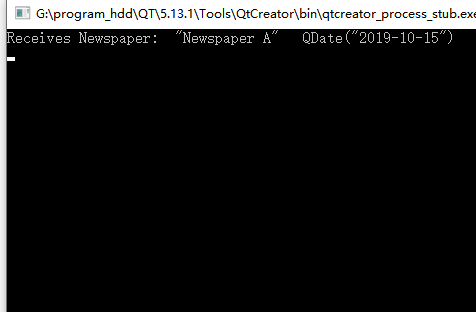
\includegraphics[width=1\textwidth]{fig/signal.png}
				\end{figure}
			\end{block}
			\pause
			\column{0.48\textwidth}
			\begin{block}{示例2-SliderSignals}
				\begin{figure}
					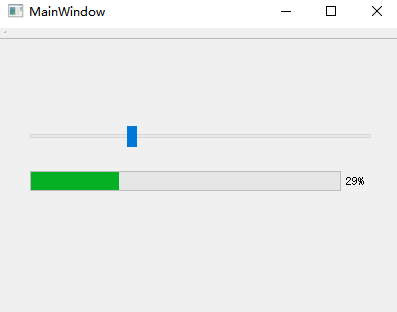
\includegraphics[width=0.83\textwidth]{fig/Slider.png}
				\end{figure}
			\end{block}
			\end{columns}
	\end{frame}
%	\begin{block}{}
%		\begin{description}
%			\item[public slots] 任何对象都可将信号与之相连接
%			\item[protected slots] 仅当前类及其子类可以将信号与之相连接
%			\item[private slots] 只有类自己可以将信号与之相连接
%		\end{description}
%	\end{block}

\begin{frame}[fragile]{2~使用Qt}
(3) 创建GUI界面
	\begin{figure}
		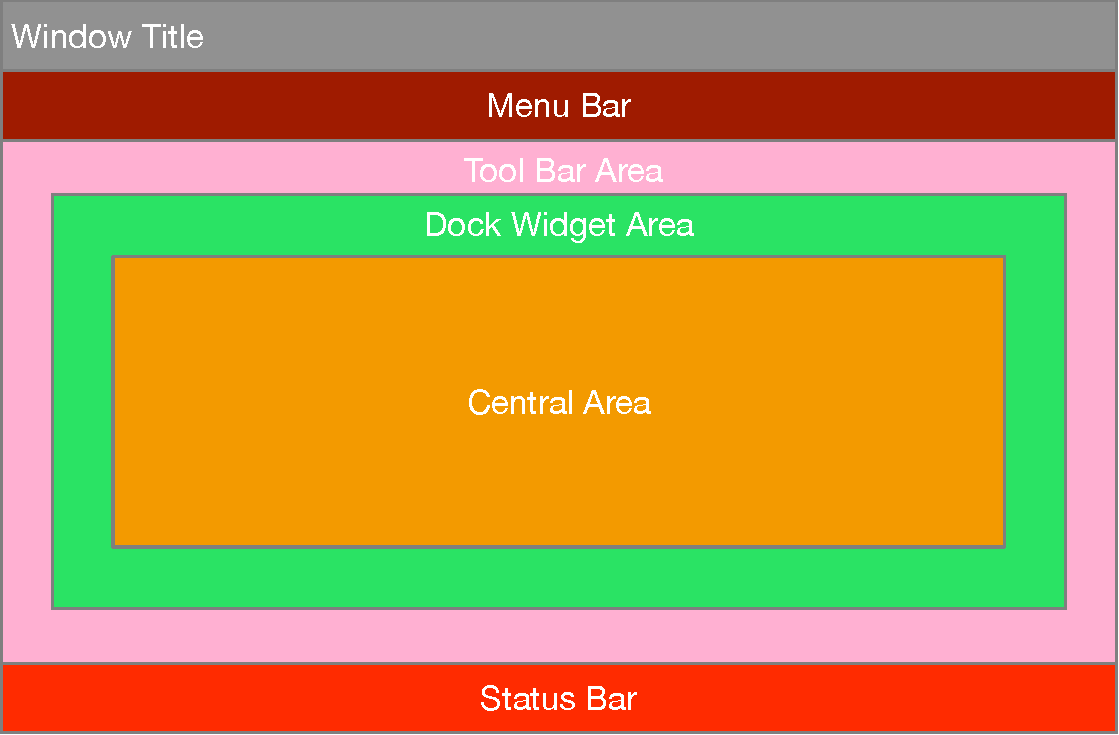
\includegraphics[width=0.6\textwidth]{fig/fig6}
	\end{figure}
\end{frame}

\begin{frame}[fragile]{2~使用Qt}
	(3) 创建GUI界面示例-Notepad
	\begin{figure}
		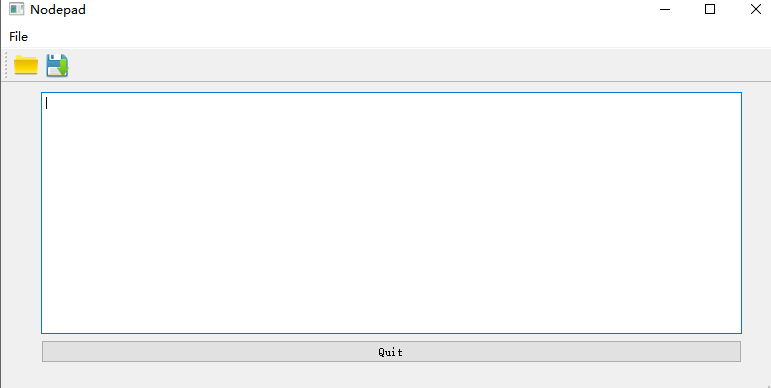
\includegraphics[width=0.7\textwidth]{fig/NotePad.png}
	\end{figure}
\end{frame}

\begin{frame}{2~使用Qt}
	(4) 动作(action)-示例
			\begin{figure}
				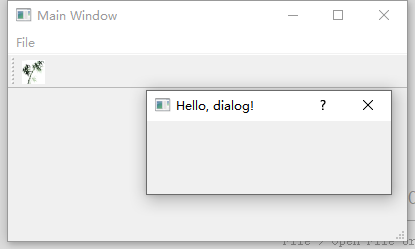
\includegraphics[width=0.5\textwidth]{fig/action.png}
			\end{figure}
\end{frame}

\begin{frame}{2~使用Qt}
(5) 使用设计模式添加控件示例-dialog
			\begin{figure}
				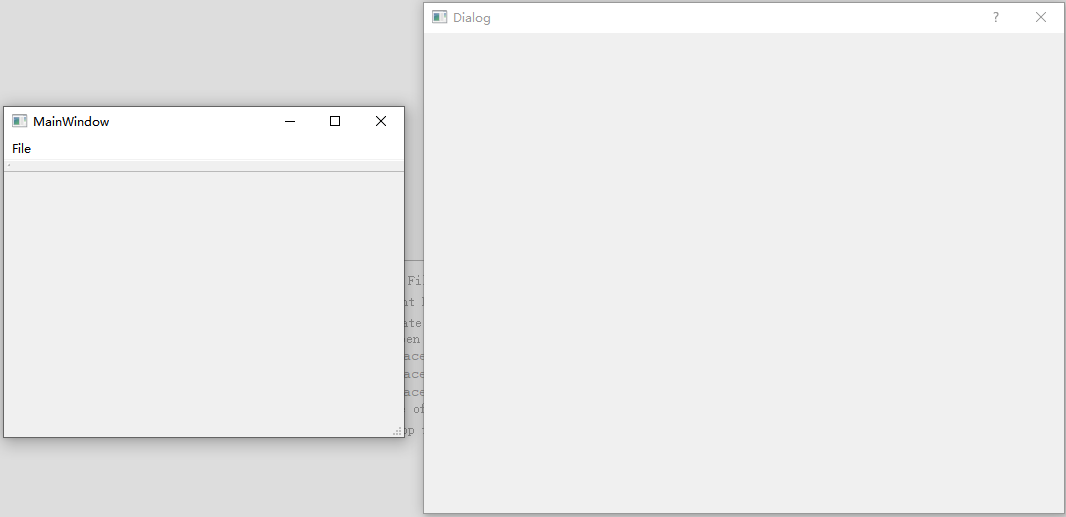
\includegraphics[width=0.7\textwidth]{fig/dialog.png}
			\end{figure}
\end{frame}

\begin{frame}[fragile]{2~使用Qt}
	(6) 使用代码编辑UI控件布局
		\begin{figure}
			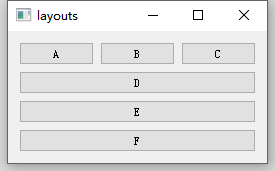
\includegraphics[width=0.45\textwidth]{fig/Layout.png}
		\end{figure}
	\end{frame}

\begin{frame}{2~使用Qt}
		(7) 事件(event)
				\begin{figure}
					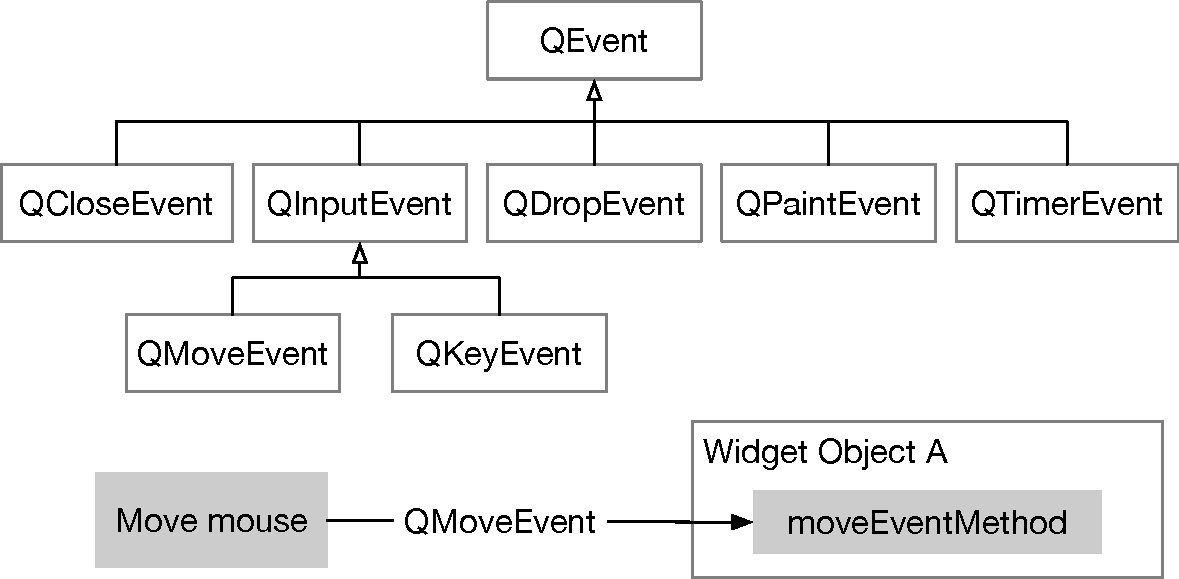
\includegraphics[width=0.75\textwidth]{fig/event.pdf}
				\end{figure}
	\end{frame}

\begin{frame}{2~使用Qt}
		(7) 事件(event)-示例
				\begin{figure}
					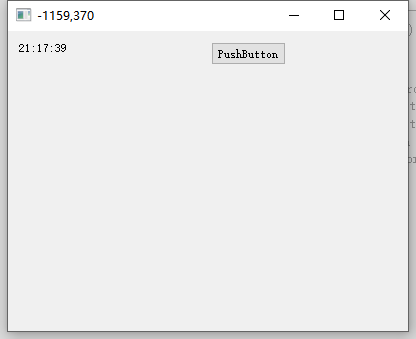
\includegraphics[width=0.5\textwidth]{fig/event.png}
				\end{figure}
\end{frame}

\begin{frame}{2~使用Qt}
	(8) 模型/视图结构(Model/View)
			\begin{figure}
				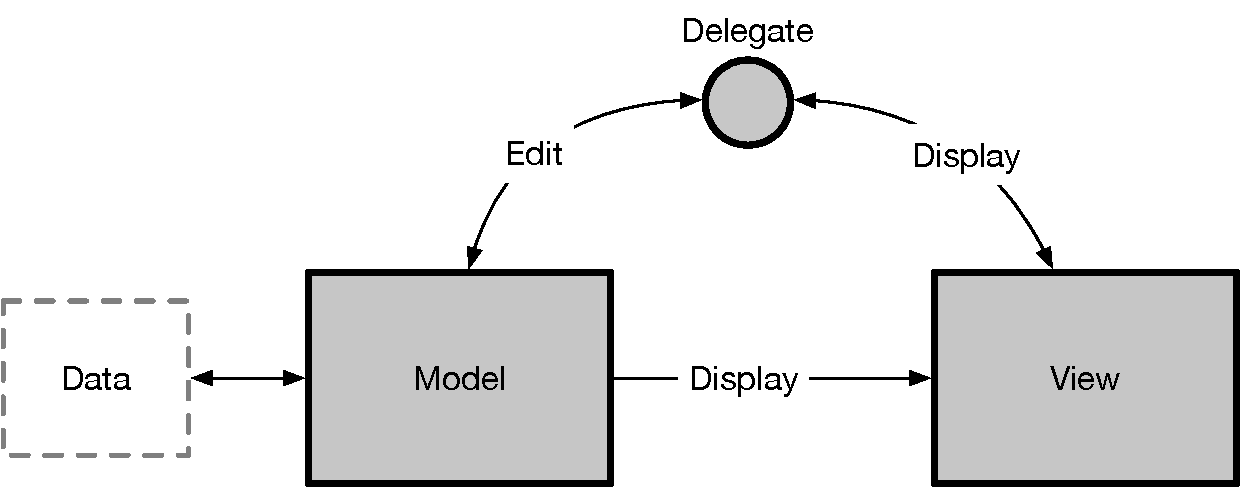
\includegraphics[width=0.7\textwidth]{fig/model_view.pdf}
			\end{figure}
\end{frame}
\begin{frame}{2~使用Qt}
	(8) 模型/视图结构(Model/View)-示例
			\begin{figure}
				\includegraphics[width=0.5\textwidth]{fig/table_view.png}
			\end{figure}
\end{frame}

\section{示例}

\begin{frame}{3~示例}
	示例一:时钟
	\begin{figure}
		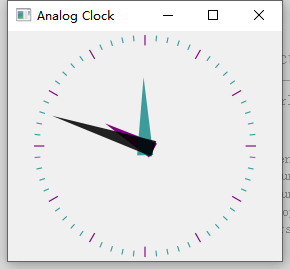
\includegraphics[width=0.4\textwidth]{fig/clock.png}
	\end{figure}
\end{frame}

\begin{frame}{3~示例}
	示例二:贪吃蛇
	\begin{figure}
		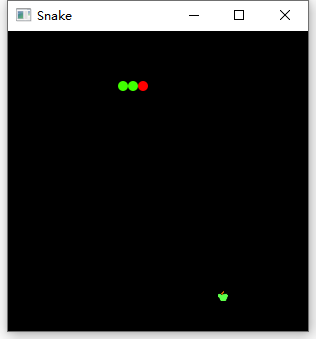
\includegraphics[width=0.4\textwidth]{fig/snake.png}
	\end{figure}
\end{frame}


\section{后记}
\begin{frame}{4~后记}

\begin{columns}[T]
\column{0.18\textwidth}
\begin{block}{C++编程风格}
\begin{itemize}
\item 数据抽象
  \item 过程化
  \item 面向对象
  \item 泛型编程
\end{itemize}
\end{block}
\column{0.3\textwidth}
\begin{block}{C++知识层级}
\begin{itemize}
  \item 层级一:语法/语意
  \item 层级二:专家经验
  \item 层级三:底层机制
  \item 层级四:设计观念的复用
\end{itemize}
\end{block}
\column{0.47\textwidth}
\vspace{2mm}

\begin{tabular}{@{}c@{~}c@{}}
 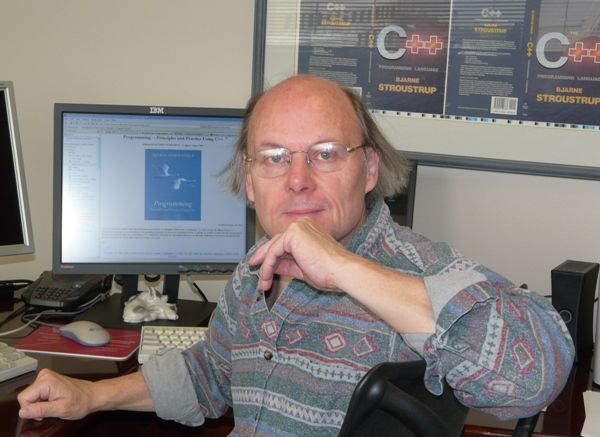
\includegraphics[width=0.55\textwidth]{fig/Bjarne.jpg} &  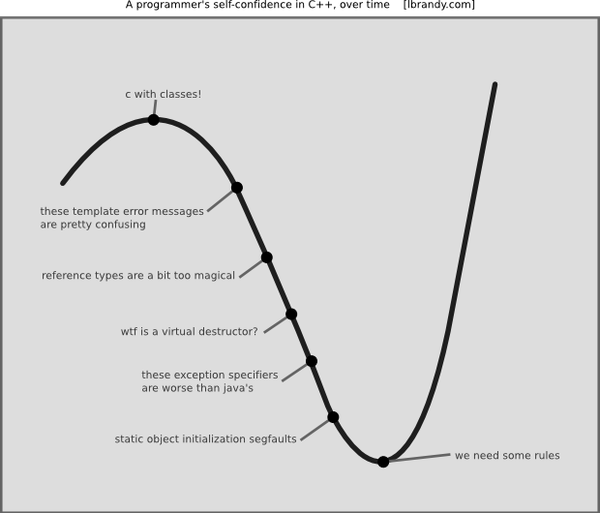
\includegraphics[width=0.48\textwidth]{fig/confidence.png}
\end{tabular}

\end{columns}
	
\begin{block}{网友的评价}
\begin{itemize}
  \item \alert{精通C++是一个艰巨的任务}。为什么C++比别的语言难学这么多?其实这基本上是因为C++他爹Bjarne Stroustrup说过的一句话“我特别讨厌语言的设计者把自己的喜好强加给用户”
C++能够自由的让你放弃某些部分,而别的语言会阻止你放弃某些部分。
  \item 谷歌工程师师对C++的掌握有两个级别:拥有C++的readability(可读性)认证;顾问级C++程序猿
  \item Never trust a programmer who says he knows C++
\end{itemize}
\end{block}
\end{frame}

\begin{frame}{4~后记}

\begin{block}{推荐C++书籍}
\begin{itemize}
\item  层级一:语法/语意(C++)
\begin{enumerate}
  \item C++ Primer ( 中文版,侯俊杰 译) by Stanley B. Lippman
\end{enumerate}
\item 层级二:专家经验(C++/OOP)
\begin{enumerate}
  \item (More )Effective C++(中文版,侯俊杰 译), by Scott Meyers.
  \item (More )Exceptional C++ (中文版,侯俊杰 译), by Herb Sutter
  \item Effective Modern C++, by Scott Meyers
\end{enumerate}
\item 层级三:底层机制(C++ Object Model)
\begin{enumerate}
\item  Inside the C++ Object Model (深度探索C++物件模型,侯俊杰 译),by Stanley Lippman.
\end{enumerate}
\item 层级四:设计观念的复用(C++/Patterns)
\begin{enumerate}
\item Design Patterns:Elements of Reusable Object Oriented Software,
by Erich Gamma,Richard Helm,Ralph Johnson,and John Vlissides
\item Modern C++ Design: Generic Programming and Design Patterns Applied by Andrei Alexandrescu.
\end{enumerate}
\end{itemize}
\end{block}
\begin{block}{编程能力}
数据结构与算法、并行编程、数据库、网络编程、图形图像与游戏
\end{block}
\end{frame}

\begin{frame}{4~后记}
\vspace{3.5cm}
\begin{center}
{\huge \color{blue} AI之路漫漫其修远兮,吾将上下而求索}
\end{center}
\end{frame}

\end{document} 